\documentclass[11pt,a4paper]{scrartcl}

%\usepackage{fullpage}

\usepackage[ngerman]{babel}
\usepackage[utf8]{inputenc}
\usepackage{graphicx}

\usepackage{amsmath}
\usepackage{amsthm}
\usepackage{mathtools}

\usepackage{listings}
\usepackage{color}

%%%%% COMMANDS

\newcommand{\FT}{\mathcal{F}}
\newcommand{\T}{\mathrm{T}}
\newcommand{\IFT}{\mathcal{F}^{-1}}
\newcommand{\conv}{\ast}
\newcommand{\defined}{\coloneqq}

\newtheorem*{theorem}{Theorem}

\renewcommand{\thesubsection}{\alph{subsection})}

 \lstset{language=C++,
basicstyle=\ttfamily,
keywordstyle=\color{blue}\ttfamily,
stringstyle=\color{red}\ttfamily,
commentstyle=\color{green}\ttfamily,
morecomment=[l][\color{magenta}]{\#},
numbers=left,
title=\lstname
}

\begin{document}

\title{Paralleles Höchstleistungsrechnen Übung 2}
\author{Markus Döring, 3153320}
\maketitle

\setcounter{section}{2}
\section{Debugging}
Das \lstinline !return! -Statement am Ende sollte natürlich die Variable \lstinline!result! zurückgeben, und nicht \lstinline!0!. 
Außerdem muss \lstinline!result! auf \lstinline!0! initialisiert werden, und darf nicht in jeder Iteration neu deklariert werden. 
\lstinputlisting[language=C++]{3.cpp}

\newpage
\section{Messen von MFLOPS}
Die C++-Programme für diese Aufgabe befinden sich im Anhang.
\subsection{}
Vgl. Abbildung \ref{fig:mflops}.
\begin{figure}[ht]
\centering
 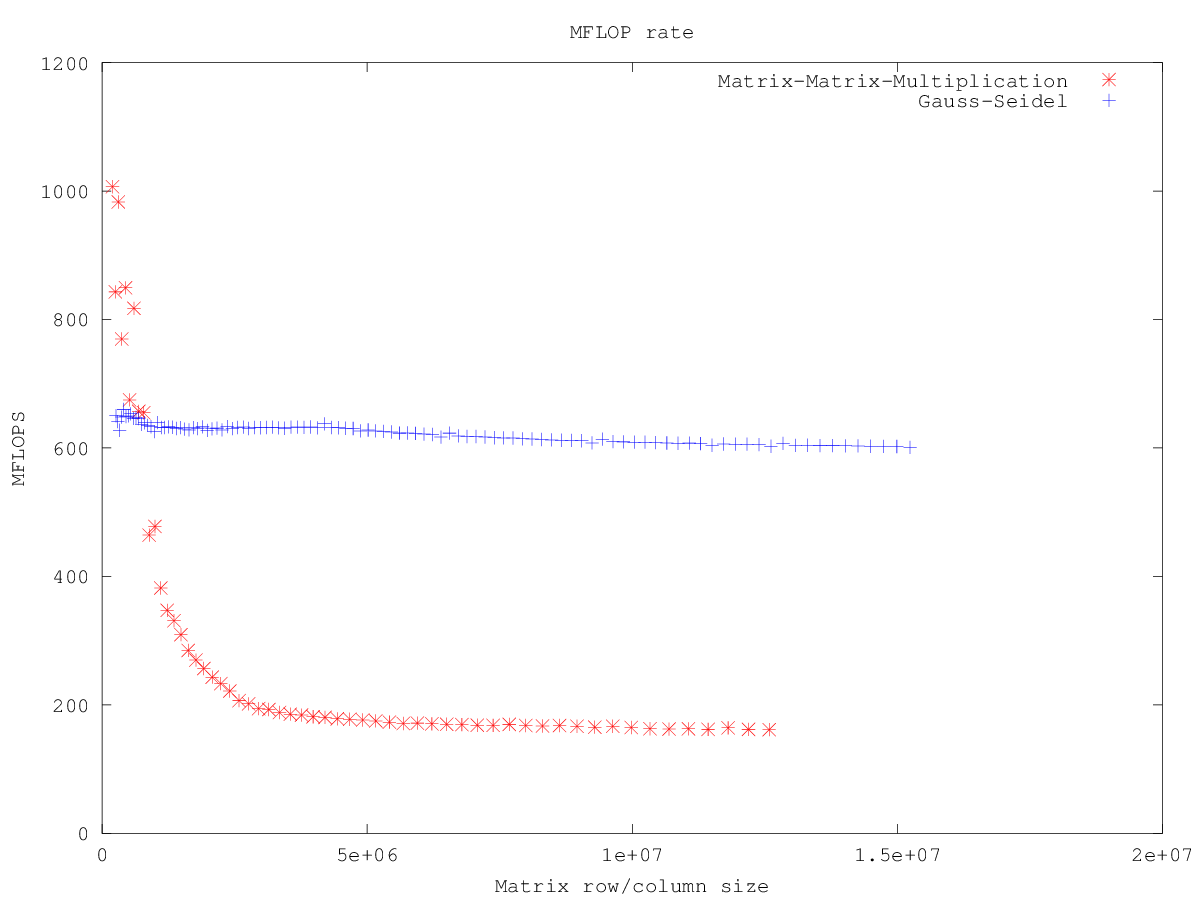
\includegraphics[width=.65\linewidth]{mflops.png}
 \caption{MFLOPS über Problemgröße. }
 \label{fig:mflops}
\end{figure}


\setcounter{subsection}{2}
\subsection{}
Vgl. Abbildung \ref{fig:tiled}.
\begin{figure}[ht]
\centering
 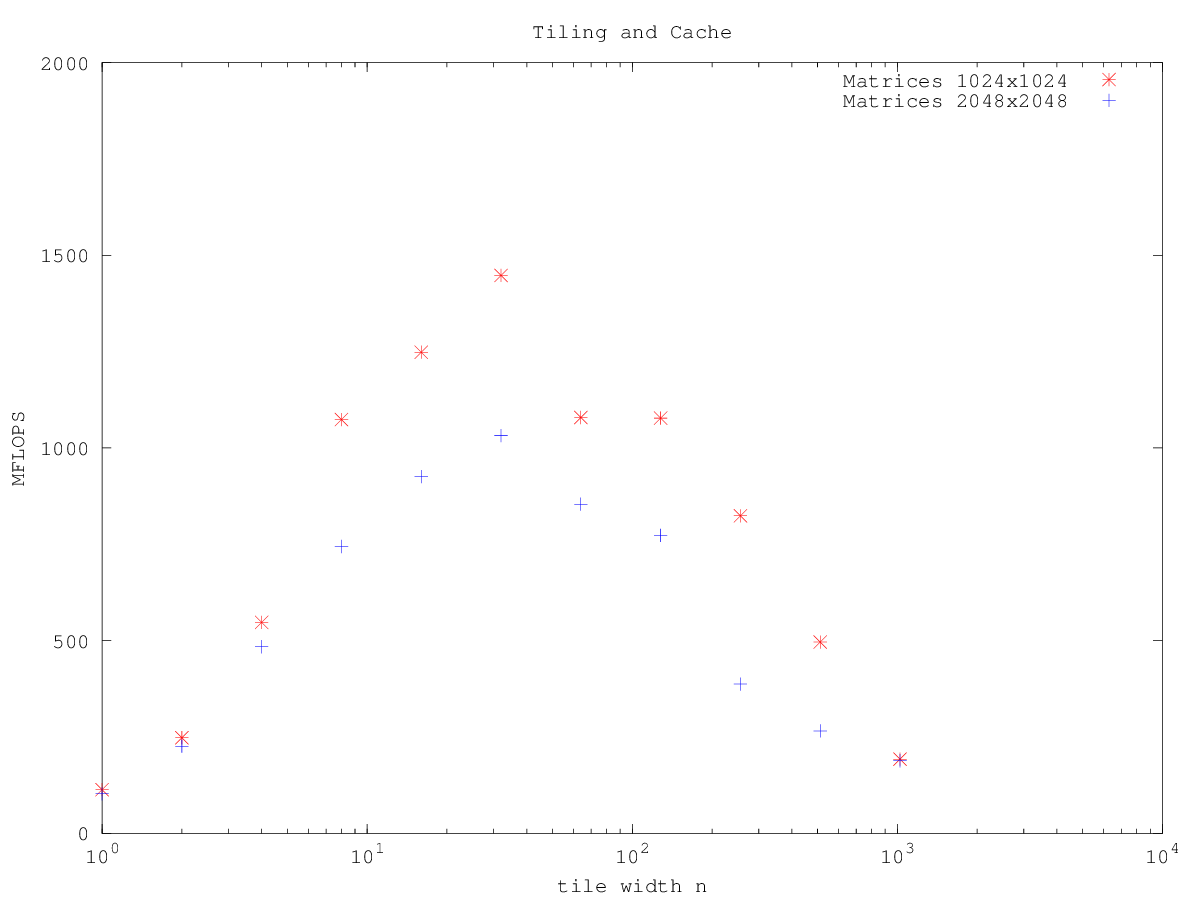
\includegraphics[width=.65\linewidth]{tiled.png}
 \caption{MFLOPS über Kachelgröße. }
 \label{fig:tiled}
\end{figure}




% \begin{figure}[ht]
%  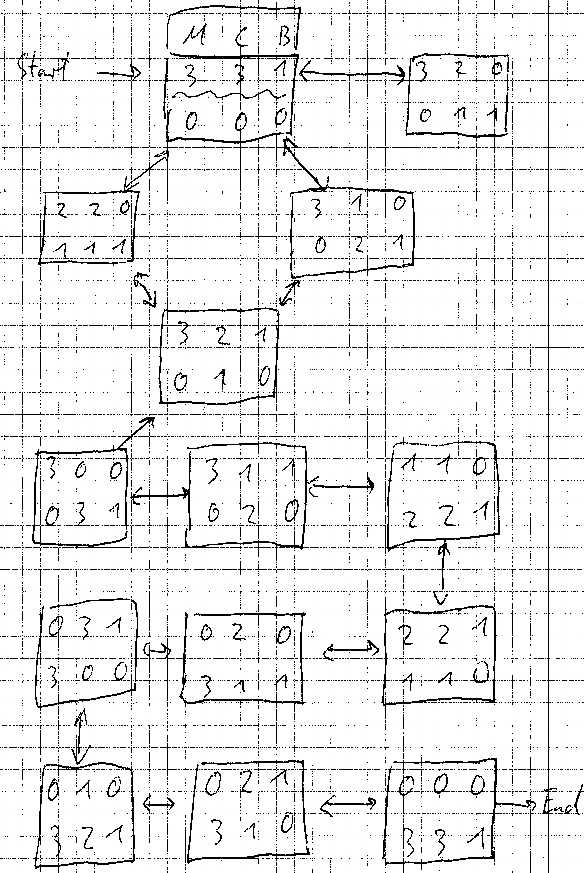
\includegraphics[width=.65\linewidth]{missionaries_cropped.jpg}
%  \caption{The state space graph of the missionary-cannibal-boat problem. The columns denote the objects (M, C, B), the rows the location (side of the river). It turns out that most possible states are not allowed by the problem statement.}
% \end{figure}

% \newpage
% \appendix
% \lstinputlisting[language=C++]{4.cpp}
%\newpage
%\lstinputlisting[language=python]{ia_05_02.py}
\end{document}
